
\FloatBarrier
\label{sec:optlayout}

\tcb{from ET design  1.3.1}

\begin{wrapfigure}{r}{0.4\textwidth}
%\begin{figure}{H}
	\centering
		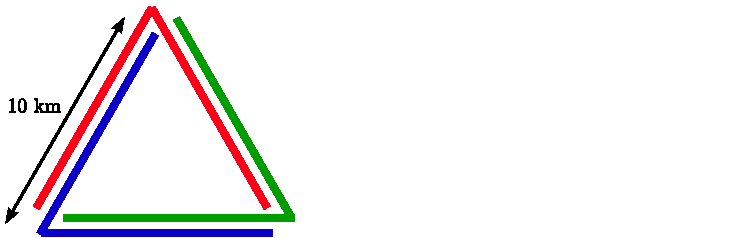
\includegraphics[width=0.3\textwidth]{Intro/Intro_Figures/NestedDetectors.pdf}
	\caption{Three nested detectors in a triangular arrangement will 
	form the final Einstein Telescope geometry.}
	\label{fig:NestedDetectors}
\end{wrapfigure}
In its final construction stage the Einstein Telescope will consist of three nested detectors, which will be arranged in a triangular pattern as shown in figure\,~\ref{fig:NestedDetectors}. In contrast to the traditional L-shaped geometry of the first and second generations of gravitational wave detectors this arrangement is equally sensitive for both polarisations of the gravitational wave. Additionally it shows a more isotropic antenna pattern compared to the L-shaped detectors, as shown in figure\,~\ref{fig:response}. The overall frequency range covered will reach from a few Hertz to about 10\,kHz.

Each individual detector in turn will comprise two interferometers, one specialised for detecting low-frequency gravitational waves and the other one for the high-frequency part. The sensitivity goal for each interferometer is shown in figure\,\ref{fig:ET_sensitivity}. %\\ 
Each individual interferometer has a classical dual-recycled Michelson topology with arm cavities. This is a mature technique, well tested in laboratory experiments, and currently being set up for the second-generation detectors, Advanced LIGO and Advanced Virgo. More elaborate topologies like Sagnac interferometers or optical bars using Quantum Non-Demolition (QND) techniques do not promise significant advantages and have not yet reached the level of  maturity required for a project of this scale.\\



\tcb{from ET design  5.4}
This section describes the details of the ET optical layout, such as the laser beam sizes, beam shapes and distances between optical components inside the arm cavities and central interferometer including the power and signal recycling cavities. A schematic sketch of the optical layout of all core optical of the interferometers is shown in figure~\ref{Fig:Simple_ETv1}.
Constraints imposed onto the optical layout are briefly discussed in section~\ref{sec:opt_layout_class}, while  section~\ref{sec:xylophone} lays out the motivation for choosing a dual-tone xylophone detector. The optical layout of the arm cavities is discussed in detail in section~\ref{sec:arm_cavity_design}. Finally section~\ref{sec:opt_layout_CITF} describes the layout of the recycling cavities. 

\begin{figure}[p]
\centering
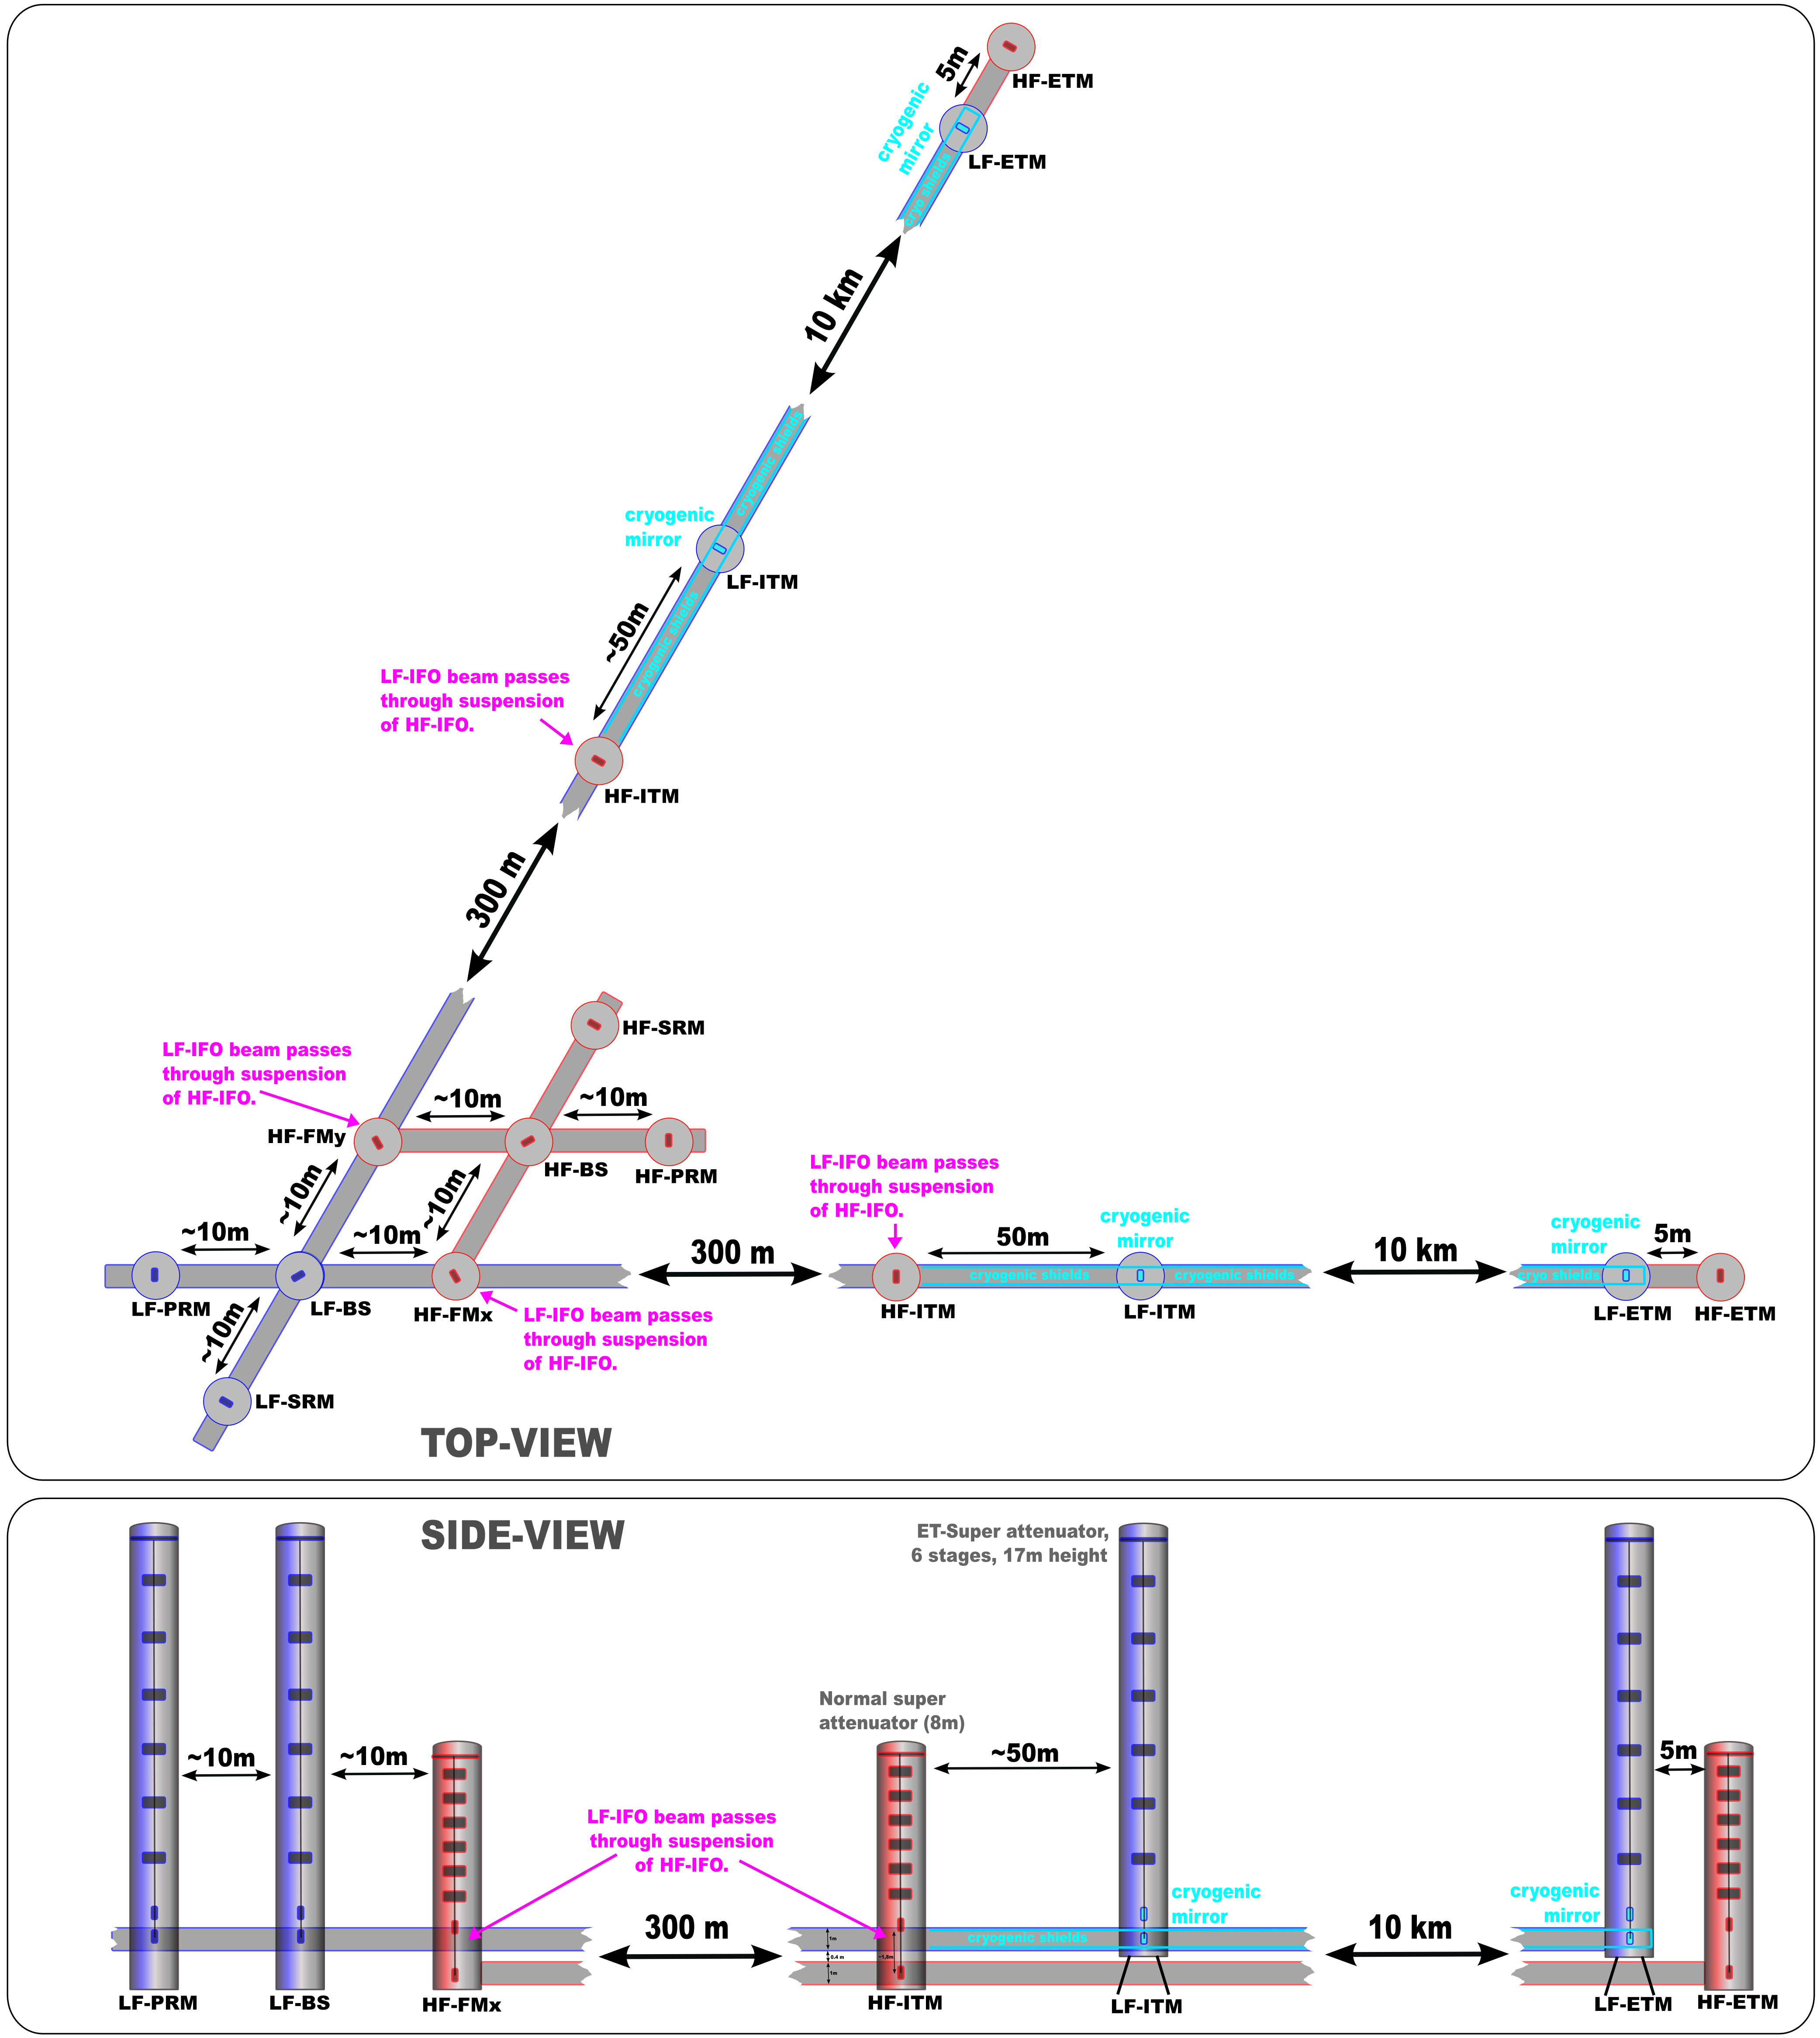
\includegraphics[width=1\textwidth]{Detector/Optics/OpticalLayout/OpticalLayoutFigures/ET_April2011_v2.png}
\caption{Simplified drawing of the low and high frequency core interferometers of a single ET-detector. Injection and detection optics as well as filter cavities have been omitted for clarity. Please not that the complete ET observatory consists of three such detectors.%
}
\label{Fig:Simple_ETv1}
\end{figure}

\subsubsection{A xylophone design for ET}\label{sec:xylophone} 
\tcb{from ET design  5.4.2}
Spanning the detection band over four orders of magnitude in frequency, as is asked for third generation GW observatories such as ET, is technically extremely challenging: different noise types dominate the various frequency bands and often show opposite responses for different tuning of the same design parameter.

In the following we give some examples of fundamental issues of a broadband third generation interferometer that could be resolved by using a set of xylophone detectors:
\begin{itemize}
\item \textbf{High Power vs Cryogenic Temperature}: Using a single broadband ET observatory as described in \cite{HildETconventional} features the challenge of the simultaneous use of high optical power (a few megawatts) to achieve the required high frequency sensitivity and test masses at cryogenic temperatures in order to provide the required suppression of thermal noise. Even though tiny, the residual absorption of the dielectric mirror coatings deposits heat in the mirrors which is difficult to extract, without spoiling the performance of the seismic isolation systems. A possible solution for this problem would be to build a xylophone observatory consisting of a high frequency detector featuring high power and high temperature and a low frequency detector featuring low power and cryogenic temperatures.
\item \textbf{Shot Noise vs Radiation Pressure Noise}: Due to the fact that the shot noise contribution scales inverse with optical power, but the photon radiation pressure noise contribution on the other hand  scales proportional to the optical power, it will be hard to obtain the desired bandwidth with a single detector. Therefore, again it might be useful to split ET into a low-power low-frequency and a high-power high-frequency
companion.
\item \textbf{Mixing Interferometer Topologies}: Xylophone configurations would also allow us to mix alternative interferometer topologies, such as Sagnac interferometer \cite{Chen2003} and optical levers \cite{Khalili2002}, with the standard Michelson interferometer. For example one could imagine that ET upgrades would feature a standard high-frequency Michelson interferometer with a low-frequency optical lever as companion.
\end{itemize}

The xylophone concept was first suggested for Advanced LIGO,  proposing to complement the standard broadband interferometers with an interferometer optimized for lower frequency, thus enhancing the detection of high-mass binary systems
\cite{Shoemaker2001LIGOXylophone, Conforto2004}.

One may think that a xylophone might significantly increase the required hardware and its cost by the need to build more than one broadband instrument. However, such an argument does not take the technical simplifications that it would allow, the better reliability of simpler instruments, and the more extensive scientific reach allowable into account.

For example splitting a third generation observatory into a low-power, low-frequency  and a high-power high-frequency interferometer, has not only the potential to resolve the above mentioned conflict of photon shot noise  and photon radiation pressure noise, but also allows to avoid the combination of high optical power and cryogenic test masses. To reduce thermal noise to an acceptable level in the low frequency band, it is expected that cryogenic suspensions and test masses are required. Even though tiny, the residual absorption of the dielectric mirror coatings deposits a significant amount of heat in the mirrors. Since this heat is difficult to extract, without spoiling the performance of the seismic isolation systems, it imposes a limit on the maximum circulating power of a cryogenic interferometer.

\begin{figure}[thbp]
\centering
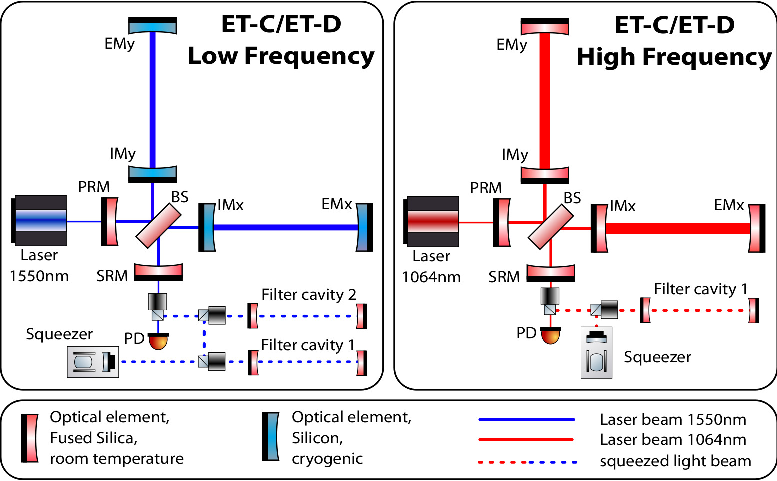
\includegraphics[width=0.8\textwidth]{Detector/Optics/OpticalLayout/OpticalLayoutFigures/Layout_overview.pdf}
\caption{Simplified sketch of the ET low and high frequency core interferometers of a single ET-detector.}
\label{Fig:opt_lay_over}
\end{figure}

\begin{table}
\begin{center}
\begin{tabular}{l l l}
\hline
\hline
Parameter & ET-D-HF   & ET-D-LF \\
\hline
Arm length & 10\,km & 10\,km \\
Input power (after IMC) & 500\,W & 3\,W \\
Arm power & 3\,MW & 18\,kW\\
Temperature & 290\,K &  10\,K  \\
Mirror material & fused silica & silicon \\
Mirror diameter / thickness & 62\,cm / 30\,cm & min 45\,cm/ T \\
Mirror masses & 200\,kg & 211\,kg \\
Laser wavelength & 1064\,nm & 1550\,nm \\
SR-phase & tuned (0.0) & detuned (0.6)\\
SR transmittance & 10\,\% & 20\,\% \\
Quantum noise suppression &  freq.\ dep.\ squeez.& freq.\ dep.\ squeez.\\
Filter cavities & $1 \times 10\,$km  & $2 \times 10\,$km\\
Squeezing level  & 10\,dB (effective) & 10\,dB (effective) \\
Beam shape &  LG$_{33}$& TEM$_{00}$\\
Beam radius & 7.25\,cm & 9\,cm \\
Scatter loss per surface & 37.5\,ppm & 37.5\,ppm \\
Seismic isolation & SA, 8\,m tall & mod SA, 17\,m tall \\
Seismic (for $f>1$\,Hz) & $5\cdot 10^{-10}\,{\rm m}/f^2$ & $5\cdot 10^{-10}\,{\rm m}/f^2$  \\
Gravity gradient subtraction & none & none \\
\hline
\hline
\end{tabular}
\caption{Summary of the most important parameters of the ET-D high and low frequency interferometers. SA~=~super attenuator,  freq.\ dep.\ squeez.~=~squeezing with frequency dependent angle.\label{tab:summary14}}
\end{center}
\end{table}

The baseline for ET is a 2-band xylophone detector configuration, composed of a low-frequency (ET-LF) and a high-frequency (ET-HF) detector. Both interferometers are Michelson interferometers featuring 10\,km armlength and an opening
angle of 60 degrees.  Due to their similar geometry both detectors will share a single facility. Table~\ref{tab:summary14} gives a brief overview of the main parameters of the analysed low-frequency (ET-LF) and high-frequency (ET-HF) detector. Figure~\ref{Fig:opt_lay_over}   shows sketches of the corresponding core interferometers and the filter cavities. The full layout of the two core interferometers of a single ET detector is depicted in Figure~\ref{Fig:Simple_ETv1}.


% -------------------------------------------------------------------------------------------
\subsubsection{Arm cavity design}
\label{sec:arm_cavity_design}
\tcb{from ET design  5.4.3}

The size and shape of the laser beam inside the interferometer is defined by the surface shape of the cavity mirrors; the beam sizes at the arm cavity input mirrors (IM) and arm cavity end mirrors (EM) as well as the position of the cavity waist are determined by only two parameters, the radii of curvature (ROC) of IM and EM. Since inside the two Fabry-Perot cavities of the Michelson interferometer the GW interacts with the laser light, creating signal sidebands, the two arm cavities can be seen as the heart of the ET interferometers. The characteristics of the arm cavities have not only a high impact on the detector sensitivity and bandwidth, but also on the overall detector performance.

The choice of the beam size on the arm cavity mirrors is a trade-off process taking the following considerations into account:
\begin{itemize}
  \item For a given cavity length there is a minimal achievable beam size, which is determined by the divergence of the beam.
\item Above this minimal beam size, any further increase in beam size leads to and additional reduction of the various thermal noise contributions.
\item Finally the upper limit for the manageable beam size is given firstly by the maximum available mirror substrate size and secondly by the approaching of the cavity instability.
\end{itemize}

\textbf{Arm cavity mirror size}

A common method to define the mirror size is to demand the optical power loss due to clipping (light being lost because it `falls over the edge of the mirror') to be less than $1\,$ppm. The computation of the scaling factors is described in~\cite{Chelkowski2009} and results in:
\begin{center}
\begin{tabular}{|l|c|c|}
	\hline
	mode  & TEM$_{00}$ & LG$_{33}$\\
	\hline
	mirror radius to beam  radius & 2.63 & 4.31\\
	\hline
\end{tabular}
\end{center}

\textbf{Minimal mirror sizes for ET}

Using the currently discussed options for ET we can compute minimal mirror sizes for various options, by using $L=R_{C}$ resulting in $w_{\rm min}=\sqrt{\frac{L\lambda}{\pi}}$.
\begin{center}
\begin{tabular}{|l|c|c|}
	\hline
setup & min beam radius  & min mirror diameter \\
         & [cm] & [cm] \\
	\hline
LG$_{33}$, 1064\,nm  &  5.8      &  50.2     \\
	\hline
TEM$_{00}$, 1550\,nm  &  7.0      &   37.0    \\
	\hline
\end{tabular}
\end{center}

\textbf{Realistic mirror sizes for ET}

Using the minimal beam sizes is obviously not optimal in terms of thermal noise. Therefore we intend to push the beam sizes for ET towards the maximum feasible size, which corresponds to about 60\,cm substrate diameter for fused silica mirrors and 50\,cm for the silicon mirrors. Assuming 10\,km long arm cavities, we can derive the following arm cavity characteristics.

\begin{center}
\begin{tabular}{|c|c|c|c|c|c|c|c|c|}
  \hline
IFO & $\lambda$& beam shape & mirror diameter & $R_{\rm C}$ & $w_0$ &$z_0$ & $w$ & $z_{\rm R}$ \\
\hline
ET-HF & 1064\,nm & LG$_{33}$ & 62\,cm & 5691\,m & 2.51\,cm & 5000\,m & 7.2\,cm & 1859\,m\\
\hline
ET-LF & 1550\,nm & TEM$_{00}$ & 45\,cm &5577\,m & 2.9\,cm & 5000\,m & 9.0\,cm & 1698\,m\\
\hline
\end{tabular}
\end{center}

% ----------------------------------------------------------------------------------------------------

\FloatBarrier
\subsubsection{Central interferometer design}
\label{sec:opt_layout_CITF}
\tcb{from ET 5.4.4 design}

The central interferometer consists of the two recycling cavities and the central Michelson interferometer formed by the beam splitter and the arm cavity input mirrors. The design of the central interferometer is mainly determined by two constraints. First of all it should allow for the implementation of non-degenerate recycling cavities. Second, the central interferometer has to serve as mode-matching telescope for the arm cavities.

The non-degenerate recycling cavity design used by the advanced detectors (see Figure~\ref{Fig:Sec_Optics_AdvLIGO_IFO_Schematic}) can probably not be directly adapted for ET, because no beam splitter substrates of the required dimensions would be available. For example the high frequency interferometer featuring an opening angle of  60 degree would require a beam splitter with a diameter of 115\,cm.

Therefore we plan to investigate design options making use of input mirror substrates including a focussing lens with a focal length of 0.2 to 1\,km and shifting the input mirrors away from the beam splitter.  Figure~\ref{Fig:Simple_ETv1} illustrates how such a configuration would look like. Please note that the arm cavity mirrors are the only full sized optical elements and that beam splitter and recycling mirrors can be significantly smaller. In addition in this scenario no additional folding mirrors are necessary in the recycling cavities.

\textbf{Layout option for TEM$_{00}$, 1550\,nm}
\nopagebreak

The optical parameters of a possible solution based on a arm cavity length of $L=10$\,km and a TEM$_{00}$ mode at 1550\,nm are provided below:
\begin{itemize}
\item focussing element in or near the ITM with a focal length of $f=303$\,m
\item distance ITM--BS: 300\,m
\item distance BS--MPR: 10\,m
\item beam size on BS: 6\,mm
\item beam size on MPR: 3.4\,mm
%\item Rayleigh range in central interferometer: 6.3\,m
\end{itemize}

The recycling cavity formed by MPR and ITM has a length of 310\,m and a free spectral range of 484\,kHz. The round-trip Gouy phase is given by $\approx 9.6$\,deg which corresponds to a mode separation frequency of $25.8$\,kHz.

\textbf{Layout option for LG$_{33}$, 1064\,nm}
\nopagebreak

Using the same distances and focussing elements for the interferometer with a LG$_{33}$, 1064\,nm beam, we also obtain reasonable numbers:
\begin{itemize}
\item beam size on BS: 4.7\,mm
\item beam size on MPR: 2.7\,mm
%\item Rayleigh range in central interferometer: 6.7\,m
\item Gouy phase: 10.5\,deg
\item mode separation frequency:  28.1\,kHz
\end{itemize}

These layout options are not yet optimised but they show that a separation between beam splitter and input optics in the order of 300\,m represents a useful baseline. The numbers for the beam sizes at the beam splitter and recycling mirrors in both cases need to be checked against a detailed thermal noise computation.

Furthermore, the design needs to be evaluated for losses originating from astigmatisms inside the recycling cavities as well as for scattered noise issues.




